\section{Performance}

To establish the performance of the final code, a comparison is made to a baseline code. In the baseline code, buses only travel, pick up and drop off passengers, and create new buses, while in the final code all the improvements described in Section \ref{sec:conceptual} are implemented.

Table \ref{table:table1} shows that there is a significant decrease in the travel time and the amount of people waiting. In the final code, more buses are added which explains the increase in bus expenses. Also, the number of messages is increased, to enable cooperation between buses. 

\begin{table*}[htbp]
\centering
\begin{tabular}{ |c|c|c|  }
 \hline
  Measurement & Baseline & Final Code \\
 \hline
  Avg travel time & 150 & 52 \\
  Buses' expenses & 1039682 & 5298614 \\
  Messages sent & 0 & 275  \\
  Final amount waiting & 232 & 25 \\
  Avg travel time remaining & 100 & 39 \\
  Final avg travel time & 156 & 54 \\
 \hline
\end{tabular}
\label{table:table1}
\caption{Performance results}
\end{table*}


From figure \ref{fig:pass_waiting} can be gathered that there is a peek in the number of passengers waiting during the morning rush hours. This peek lowers, when more buses are added. Thanks to the enlarged bus fleet, a much smaller peek is seen during the second rush hour in the evening.

See figure \ref{fig:expense}
see figure \ref{fig:messages}
See figure \ref{fig:avg_tt}

\begin{figure}[htbp]
\centering
\begin{minipage}{.48\textwidth}
  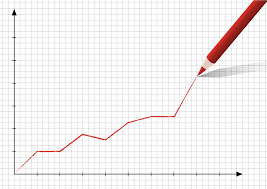
\includegraphics[width=.4\textwidth]{src/expenses.jpg}
  \caption{\label{fig:expense}Figure that displays the expenses of the buses.}
\end{minipage}%
\begin{minipage}{.48\textwidth}
  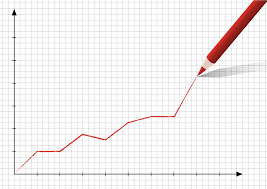
\includegraphics[width=.4\textwidth]{src/nr_messages.jpg}
  \caption{\label{fig:messages}Figure that displays the number of exchanged messages.}
\end{minipage}
\end{figure}

\begin{figure}[htbp]
\centering
\begin{minipage}{.48\textwidth}
  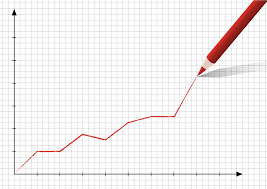
\includegraphics[width=.4\linewidth]{src/nr_pass_waiting.jpg}
  \caption{\label{fig:pass_waiting}Figure that displays the number of passengers waiting.}
\end{minipage}%
\begin{minipage}{.48\textwidth}
  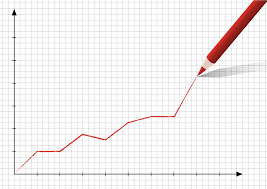
\includegraphics[width=.4\linewidth]{src/avg_tt.jpg}
  \caption{\label{fig:avg_tt}Figure that displays the average travelling time.}
\end{minipage}
\end{figure}
